%% CAV 2017

% Deadlines:
% papers due : Jan 24, 2017
% (lncs format, 16 pages max excluding appendix and references)

%%%%%%%%%%%%%%%%%%%%%%%%%%%%%%%%%%%%%%%%%

\documentclass[letterpaper]{llncs}
\pagestyle{headings}
\usepackage{amssymb}
\usepackage{graphicx}
\usepackage{url} 
\usepackage{float}

\newcommand{\keywords}[1]{\par\addvspace\baselineskip
\noindent\keywordname\enspace\ignorespaces#1}
\newcommand{\eg}{\mbox{\em e.g.}}
\newcommand{\viz}{\mbox{\em viz.}}

\usepackage{setspace}
\usepackage{algpseudocode}
\usepackage{algorithm}
\usepackage{soul}
\usepackage{amsmath}
\usepackage{amssymb}
\renewcommand{\labelitemi}{\tiny$\blacksquare$}

\newlength\myindent
\setlength\myindent{2em}
\newcommand\bindent{
  \begingroup
  \setlength{\itemindent}{\myindent}
  \addtolength{\algorithmicindent}{\myindent}
}
\newcommand\eindent{\endgroup}

\begin{document}

\mainmatter  % start of an individual contribution

\title{Formal Verification Techniques for Behaviorally Synthesized Loop Pipelines}

% the name(s) of the author(s) follow(s) next
\author{Disha Puri\inst{1}
\and Sandip Ray\inst{2} 
\and Fei Xie\inst{1}
\and Kecheng Hao\inst{1}} 

\institute{Department of Computer Science, Portland State University, Portland, OR 97207.
\and
NXP Semiconductors}

\maketitle
\begin{abstract}
\label{sec:abstract}

Behavioral Synthesis is the process of compiling an Electronic System Level (ESL) design in high-level languages such as C, C++ or SystemC into Register-Transfer Level (RTL) implementation in hardware description languages such as Verilog or VHDL.
Loop pipelining is a critical transformation in this process, which improves
the throughput and reduces the latency of the synthesized hardware. It is
complex and error-prone, and a small bug can result in faulty hardware with expensive
ramifications. Therefore, it is critical to certify the loop pipelining transformation
so that designers can trust the behavioral synthesis process.
Certifying a loop pipelining transformation is however, a major research challenge
because there is a huge semantic gap between the input sequential design and the output
pipelined implementation, making it infeasible to verify their equivalence with automated sequential equivalence
checking (SEC) techniques.

Certification of a loop pipelining transformation is possible by a combination of theorem
proving and SEC: (1) creating a certified pipelining algorithm which generates a reference
pipeline model by exploiting pipeline generation information from the synthesis flow ({\em e.g.},
the iteration interval of a generated pipeline) and (2) conduct SEC between the synthesized pipeline
and this reference model. A key and arguably, the most complex component of this
approach is development of the certified
loop pipelining algorithm. We propose a framework of certified pipelining primitives which we show
are essential for designing pipelining algorithms. Using our framework, we build
a certified loop pipelining algorithm. We also propose a key invariant in certifying this algorithm, which links sequential loops
with their pipelined counterparts. This is unlike other invariants that have been used in pipeline proofs.

The result of this dissertation is a framework for creating certified pipelining algorithms
utilizing a mechanical theorem prover. Using this framework, we have developed a certified loop pipelining
algorithm. This certified algorithm is essential in the overall approach to certify
behaviorally synthesized pipelined designs. We test the scalability and robustness of our algorithm on
industrial-strength ESL designs that result in tens of thousands of lines of RTL implementations.
     
\end{abstract}

\section{Introduction}
\label{sec:intro}

In recent years, the demand for hardware with smaller form factor and higher transistor density has been steadily increasing. Consequently, it has become difficult to create high quality hardware by hand-crafting RTL designs. A behavioral synthesis tool takes a behavioral
%n implementation independent 
design description (in C, C++, or SystemC), often referred to as Electronic System Level (ESL) design, and automatically generates an optimized RTL design (in hardware
description languages such as VHDL or Verilog). Industrial users
have found that behavioral design reduces the design effort
by 50\% or more while attaining excellent performance results~\cite{Moussa99}. However, the adoption of this approach is
contingent upon certifying that the RTL design indeed
corresponds to the ESL description.

Loop pipelining is one of the most complex transformations in behavioral synthesis. It is available in most commercial synthesis tools ({\em e.g.}, AutoESL~\cite{autoesl} and Cynthesizer~\cite{forte}) and is
crucial to producing hardware with high throughput and low latency by allowing temporal overlap of successive loop
iterations. Certifying the correspondence between a sequential design and its pipelined counterpart is challenging due to the huge semantic gap between the two
designs.

We develop a framework for designing certifiable
pipelining algorithms. It has three pipelining primitives on which one can build a pipelining algorithm. In particular, using our framework, we develop a certifiable
loop pipelining algorithm that can be used for certifying a pipeline generated by a behavioral synthesis tool. Our algorithm takes a sequential design as input,
together with certain parameters readily available from a behavioral synthesis tool and produces a pipeline reference
model. It has been shown that such a reference model can be verified with the pipelined RTL using sequential equivalence checking (SEC)~\cite{hrx:dac-12}.

%We develop a framework to create certifiable pipeline generation algorithms. We identify three pipelining primitives which have the potential to affect the correctness of a design while pipelining. We show how to create a simple loop pipeline generation algorithm using our framework. The algorithm takes sequential design and pipeline interval (obtained from the behavioral synthesis tool) as input and produces a pipeline reference model. 

%The reference model can then be verified with the pipelined RTL using Sequential Equivalence Checking~\cite{hrx:dac-12}. It is possible because the reference model is created using feedback from the synthesis tool, so it is structurally similar to the pipelined RTL. An algorithm was proposed in an earlier paper ~\cite{hrx:dac-12} to create the pipeline reference model and was tested on a behavioral synthesis tool, AutoESL. However, the proposed algorithm was not certified.

\medskip
The key contributions of this paper are:
\begin{enumerate}
\item a framework of three pipelining primitives to create certifiable pipelining algorithms;
\item a simple certifiable loop pipelining algorithm using our framework; and 
\item a proof methodology for mechanically certifying such an algorithm using a theorem prover.
\end{enumerate}

%Note that we choose not to certify the algorithm proposed by Hao et al.~\cite{hrx:dac-12} because we believe it would be a messy and difficult proof. Also, one of our key insights is that while the certification framework requires an algorithm that generates pipeline reference model that can be used for SEC with RTL produced by synthesis tools, we are free to choose an implementation of the transformation amenable to formal reasoning. 

The rest of the paper is organized as
follows. Section~\ref{sec:background} provides relevant background and an uncertified algorithm to generate
pipelines. Section~\ref{sec:not-verifiable} explains our motivation behind developing the framework. Section~\ref{sec:fundamental-tasks} explains the primitives for creating certifiable
pipelining algorithms in behavioral
synthesis. Section~\ref{sec:pipeline-algo} presents a simple certifiable pipelining algorithm using these primitives. Section~\ref{sec:proof}
explains our approach to certify the primitives. Section~\ref{sec:related} explains related work and Section~\ref{sec:concl} concludes this paper and discusses future work.

%Verifying a complex pipelined design by standard sequential equivalence checking (SEC) does not work. Equivalence checking requires mapping of internal operations and variables in the two design per clock cycle. Loop pipelining produces a new schedule and a different control flow as compared to sequential design as more than one iterations are being done in parallel in a single clock cycle. To avoid data hazards (overwrite of variables before being read), new variables are introduced in the pipelining process. Due to all this, mapping of internal operations between sequential and pipelined design is lost making SEC infeasible. Since, tool vendors do not disclose their implementation of pipelining transformation, certification by theorem proving is also ruled out.


\section{Background and Context}
\label{sec:background}


%% We represent the
%% intermediate representation in the form of a Clocked Control
%% Data Flow Graph and use LLVM language. Both these choices do
%% not add any unnecessary complexity to our formal
%% reasoning. We now provide an overview of our intermediate
%% representation and the loop pipelining transformation done
%% in behavioral synthesis tools.

\subsection{Intermediate Representation}
\label{subsec:ir}

%We represent the intermediate design in the form of a Clocked Control Data Flow Graph (CCDFG)~\cite{rhcxy:atva-09}. 
A behavioral synthesis tool performs a number of compiler
and scheduling transformations (including pipelining, which is the focus of this paper). Certification of behavioral
synthesis transformations thus requires a formalization of
the design representation manipulated by these
transformations. The formalization we use is {\em Clocked
  Control Data Flow Graph} (CCDFG)~\cite{rhcxy:atva-09}. It
is a natural formalization of an intermediate design
representation used by most behavioral synthesis tools.
Structurally, a CCDFG is a control and data flow graph augmented with a schedule.
% We use a structure called CCDFG to formalize internal
% respresentations of designs generated by behavioral
% synthesis tools(CCDFG)~\cite{rhcxy:atva-09}. Thus, our
% algroithm accepts CCDFG for sequential design and
% generates a pipelined CCDFG. A CCDFG is a Control Data
% Flow Graph augmented with a schedule.
The control flow is broken into basic blocks. The instructions are grouped into microsteps which can be executed concurrently. A scheduling step represents a group of microsteps which can be executed in a single clock cycle. State of a CCDFG at a particular microstep is a list of all the variables of a CCDFG with their corresponding values. 
%% CCDFG is a
%% natural formalization of internal representation structure
%% used in behavioral synthesis tools.

The semantics of CCDFG require a formalization of the
underlying language used to represent the individual
instructions in a scheduling step.  The underlying language we use
is the LLVM language~\cite{llvm}. LLVM is a popular compiler
infrastructure for many behavioral synthesis tools
({\em e.g.}, AutoESL~\cite{autoesl}, xPilot~\cite{xpilot},
LegUp~\cite{legup}).  We provide semantics to these
instructions through a standard, state-based operational
formalization~\cite{McCarthy}. It includes assignment,
load, store, bounded arithmetic, bit vectors, arrays, and
pointer manipulation instructions. Executing a microstep in
a CCDFG implies changing the current state of CCDFG based on
meaning of the instructions in the microstep and producing a
new state. Assigning meanings to most instructions is
standard; one exception is the so-called ``$\phi$-construct''. A $\phi$-construct is a list of $\phi$-statements. A $\phi$-statement is $v := \phi [\sigma, X] [\tau, Y]$, where $v$ is a variable, $\sigma$
and $\tau$ are expressions, and $X$ and $Y$ are
scheduling steps: if it is reached from $X$ then it is the
same as the assignment statement $v := \sigma$; if
reached from $Y$, it is the same as $v := \tau$; the meaning is undefined otherwise. $\phi$-constructs are necessary due to the structure of the SSA (static single
assignment) form of the LLVM code.

\subsection{Loop Pipelining Transformation}
\label{subsec:loop-pipelining-trans}
A behavioral synthesis tool automatically generates a RTL design from an ESL design through a series of
transformations. Pipelining a loop is a critical
transformation in behavioral synthesis. For our purposes, a
{\em pipelinable loop} is a loop with the following additional restrictions~\cite{hrx:dac-12}:
\begin{enumerate}
\item no nested loop;
\item only one $Entry$ and one $Exit$ block; and
\item no branching between the scheduling steps.
\end{enumerate}
These restrictions reflect the kind of loops that can be
actually pipelined during behavioral synthesis. For
instance, synthesis tools typically require inner loops to
have been fully unrolled (perhaps by a compiler
transformation) in order to pipeline the outer loop.


\begin{figure}[H]%[t!]
\begin{center}
\begin{tabular}{cc}
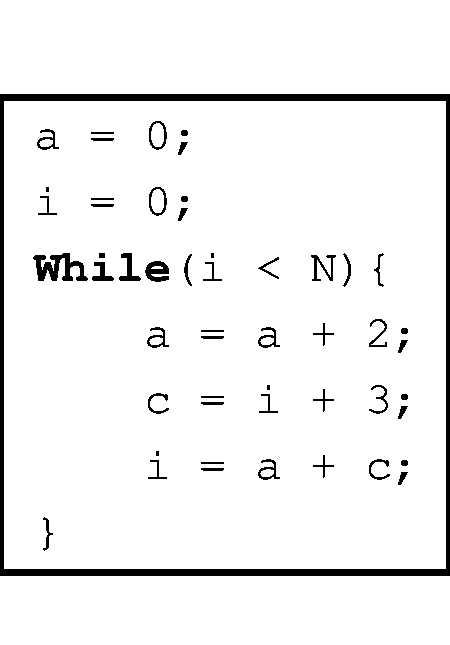
\includegraphics[height=1.8in]{fig-rpe/C-code}
& \hspace{2cm}
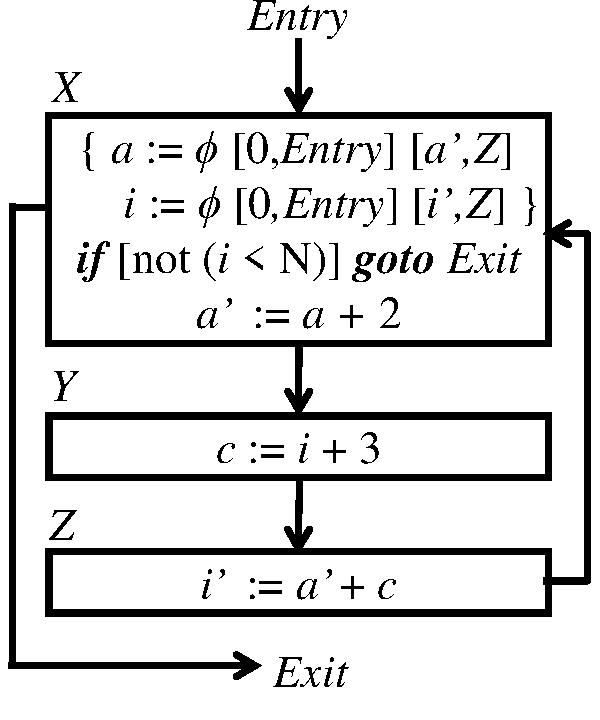
\includegraphics[height=1.8in]{fig-rpe/seq-ccdfg}
\\
(a) & \hspace{2cm} (b) 
\end{tabular}
\end{center}
\caption{(a) Loop in C (b) Loop CCDFG before pipelining.}
\label{fig:high-level-synthesis}
\end{figure}

Figure~\ref{fig:high-level-synthesis}(a) illustrates the C
code (ESL description) for a loop at the beginning of the
synthesis process. The C code does not have a schedule or the
concept of a clock cycle. Figure~\ref{fig:high-level-synthesis}(b)
shows CCDFG of the sequential loop just before loop pipelining. The loop has three scheduling steps: $X$, $Y$ and $Z$.  The scheduling step before the loop is $Entry$ and after the loop is $Exit$. Since,
there are three scheduling steps in the loop, one iteration
can be executed in three clock cycles.

\begin{figure}
\begin{center}
\begin{tabular}{cc}
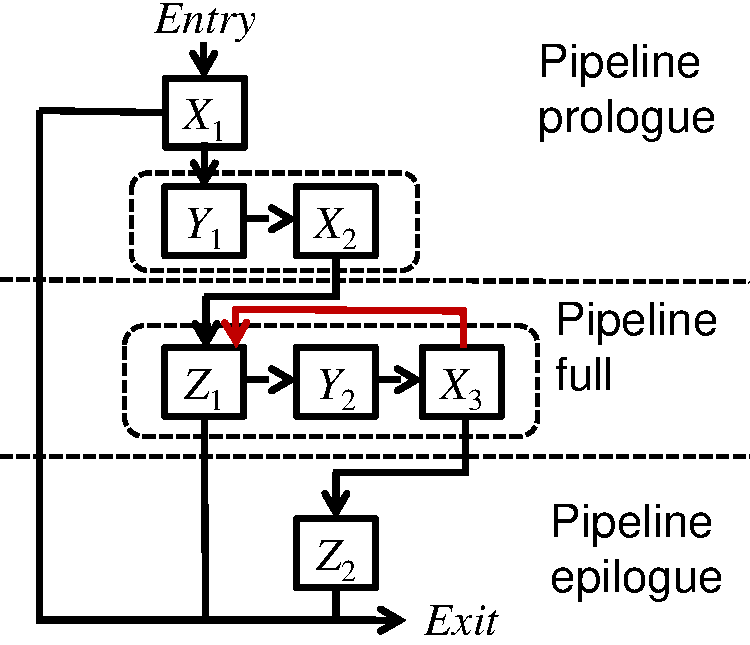
\includegraphics[height=1.8in]{fig-rpe/pipelined_ccdfg}
& \hspace{0.5cm}
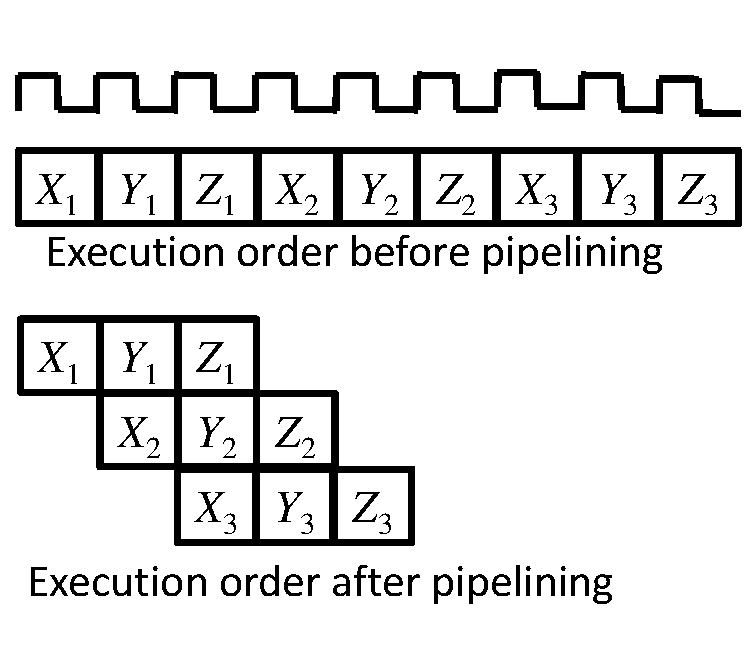
\includegraphics[height=1.8in]{fig-rpe/pp-clock-cycles}
\end{tabular}
\end{center}
\caption{Pipelined CCDFG. The horizontal arrows in the scheduling supersteps indicate data forwarding.}
\label{fig:pp-ccdfg}
\end{figure}

Behavioral synthesis tools use complicated heuristics and aggressive scheduling strategies to find an optimized pipeline interval (clock cycles after which a new iteration can be started such that there are no data hazards). Figure~\ref{fig:pp-ccdfg} shows the pipelined CCDFG with a pipeline interval equal to one. The new scheduling steps in the pipelined CCDFG created by combining scheduling steps from different iterations of the sequential CCDFG are called scheduling supersteps. Observe that the three iterations of the pipelined loop take five clock cycles as opposed to nine clock cycles in the sequential loop. Loop pipelining reduces the number of clock cycles required to execute the loop, hence this transformation is used by synthesis tools to increase throughput and reduce latency.  

\subsection{Correctness of Pipelined CCDFG}
\label{subsec:correctness-defn}

Loop Pipelining is a critical and complex transformation. So, it is important to certify that the pipelined CCDFG is indeed correct. Correctness of loop pipelining 
can be informally stated as below.

\begin{quote}
Let $L$ be a loop in CCDFG $C$, and let $L_{\alpha}$ be the
pipelined loop CCDFG. Let $V$ be the set of
variables mentioned in $L$, and $U$ be the set of all
variables in $C$.  Suppose we execute $L$ and $L_{\alpha}$
from CCDFG states $s$ and $s'$ respectively, such that for
each variable $v\in V$, the value of $v$ in $s$ is the same
as that in $s'$, and suppose that the state on termination
are $f$ and $f'$ respectively.  Then (1)~for any $v\in V$,
the value of $v$ in $f$ is the same as that in $f'$, and
(2)~for any $v\in(U\backslash V)$, the value of $v$ in $f'$
is the same as that in $s'$.
\end{quote}
\noindent
{\em Remark:} Condition (2) is the {\em frame rule} which
ensures that variables in $C$ that are not part of the loop
are not affected by $L_{\alpha}$.

\subsection{An approach to verification of loop pipelining transformation}
\label{subsec:hao-approach}

%Hao et al.~\cite{hrx:dac-12} develop a pipeline algorithm that takes as inputs these parameters and a CCDFG and generates a reference pipelined CCDFG. 
Hao {\em et al.} proposed a pipeline generation algorithm using feedback (like pipeline interval) from the synthesis tool~\cite{hrx:dac-12}. They show that to verify the correspondence between sequential CCDFG and pipelined RTL, it is sufficient to perform the following three steps. 
\begin{enumerate} 
\item Check that the algorithm can generate a pipeline reference model for the parameters reported by synthesis.
\item Use SEC to compare the pipeline reference model with the
synthesized RTL.
\item Prove the correctness of the algorithm. 
\end{enumerate}

The pipelining algorithm is simpler than that used by the synthesis tool because the synthesis tool uses advanced heuristics to determine the pipeline parameters 
(such as how many iterations to pipeline, when to introduce stalls etc.), while this pipelining algorithm only uses those parameters to generate a reference model. The algorithm is shown to be scalable but it is not certified. 

\medskip
\noindent {\bf The proposed algorithm}
\label{subsec:kecheng's algorithm}

\noindent
Given a set of microsteps $M$, a set of edges $E$, and a schedule $S$ of a
sequential CCDFG, and pipeline parameters (pipeline
interval $I$ and number of scheduling steps in the loop
$N$), the algorithm generates new microsteps, edges and
schedule for pipelined CCDFG by pipelining the
loops. Values of these inputs are readily available from
intermediate feedback reports from the behavioral synthesis
tool. Given CCDFG $C$, the reference transformation replaces
each loop $L$ in $C$ with the pipelined refinement of
$L$. The steps of the algorithm are explained below with the
help of the example introduced earlier
(cf. Figure~\ref{fig:high-level-synthesis}) .

%\medskip
%\begin{algorithm}
%\caption{Loop Pipelining Algorithm} \label{algo:hao}
%\begin{algorithmic}[1]
%\Procedure{PIPELINELOOP}{L=(S, E, M), I, N}
%\State $S_1 \leftarrow Generate Scheduling Steps (S, I, N)$.
%\State $(S_2, M_1) \leftarrow Generate Pipeline Regs (S_1, M, E, I)$.
%\State $ E_1 \leftarrow Generate Edges (S_2, E, I, N)$.
%\State $S_3, M_2) \leftarrow Generate Forwarding (S_2, M_1, E_1, I)$.
%\State \textbf{return} $(S_3, E_1, M_2)$.
%\EndProcedure
%\end{algorithmic}
%\end{algorithm}

\begin{figure}
\begin{center}
\begin{tabular}{cc}
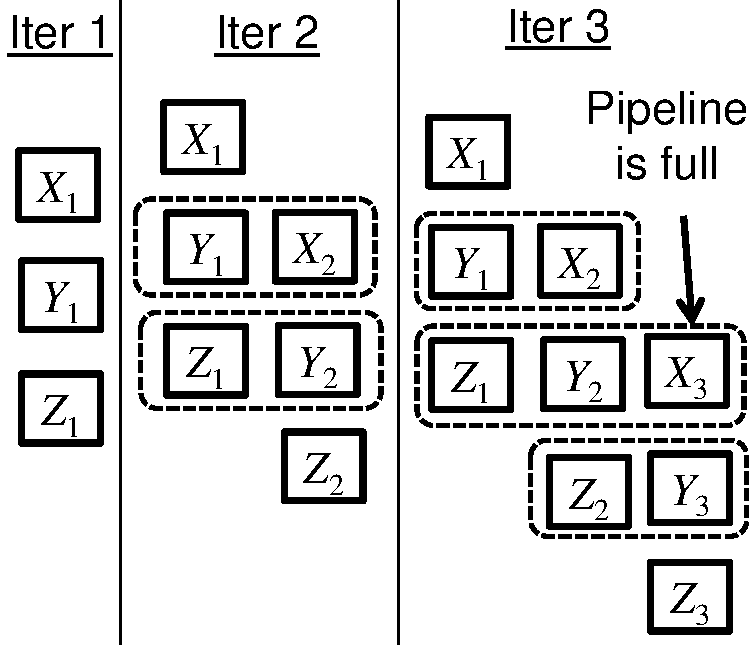
\includegraphics[height=1.7in]{fig-rpe/generate-scheduling-steps}
& %\hspace{0.1cm}
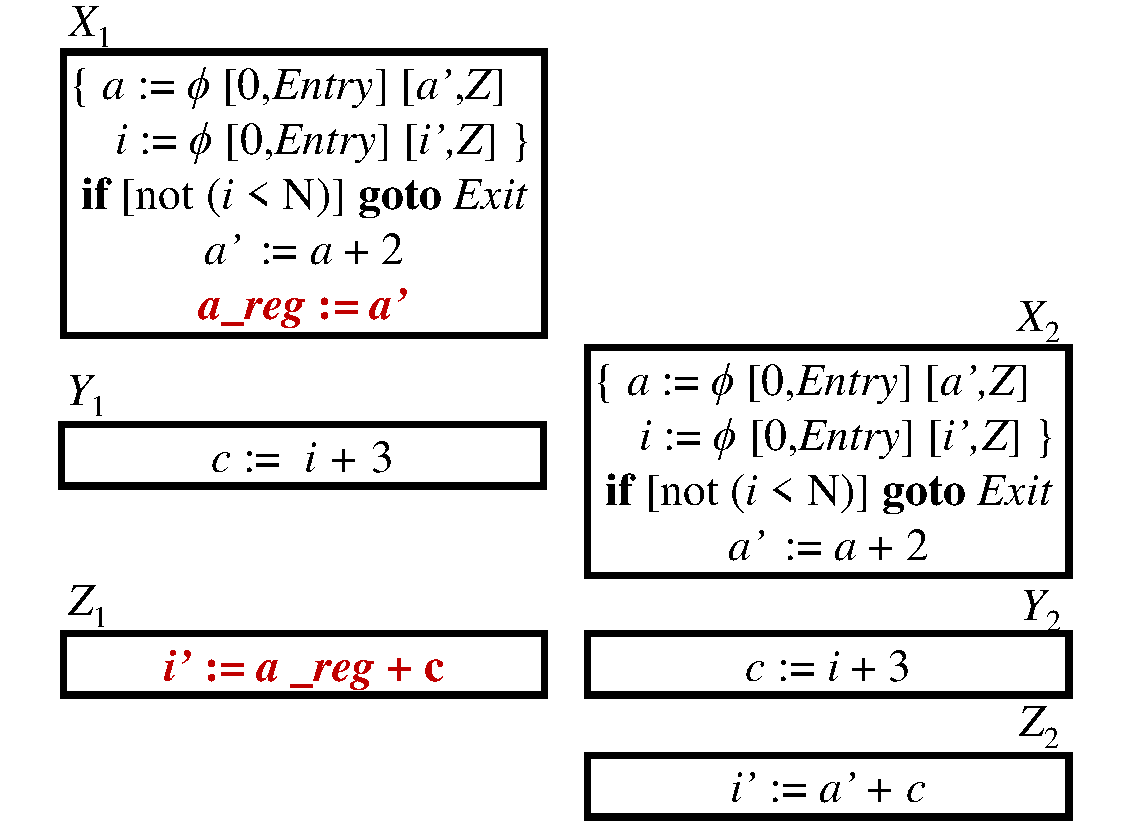
\includegraphics[height=1.7in]{fig-rpe/shadow-reg}
\\
(a) & (b)
\end{tabular}
\end{center}
\caption{(a) Generate scheduling steps. After the pipeline is full, adding new iteration simply repeats the pipeline full stage. (b) Generate shadow registers.}
\label{fig:algorithm}
\end{figure}

\begin{enumerate}
\item {\bf Generate scheduling steps:} Figure~\ref{fig:algorithm}(a) shows the addition of scheduling steps of new iterations of a loop according to the pipeline interval. Here, the loop has three scheduling steps and a pipeline interval of one. The new scheduling steps are generated till the pipeline is full. This step generates a new schedule. 

\item {\bf Generate shadow registers:} In order to pipeline a loop, we have to get rid of data hazards. We first identify all variables that can be overwritten and then introduce new variables called shadow registers. In Figure~\ref{fig:algorithm}(b), the value of $a'$ will be overwritten in $X_2$ before $Z_1$ can read it. So, we introduce a new pipeline register $a\_reg$ which gets assigned the value of $a'$ and replace subsequent reads of $a'$ with reads of $a\_reg$.

\begin{figure}[t!]
\begin{center}
\begin{tabular}{cc}
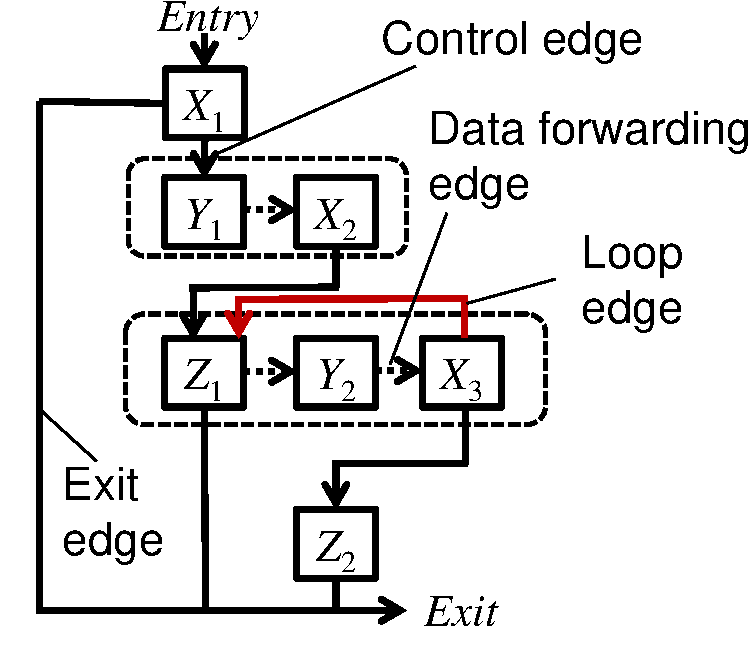
\includegraphics[height=1.7in]{fig-rpe/generate-edges}
& %\hspace{0.1cm}
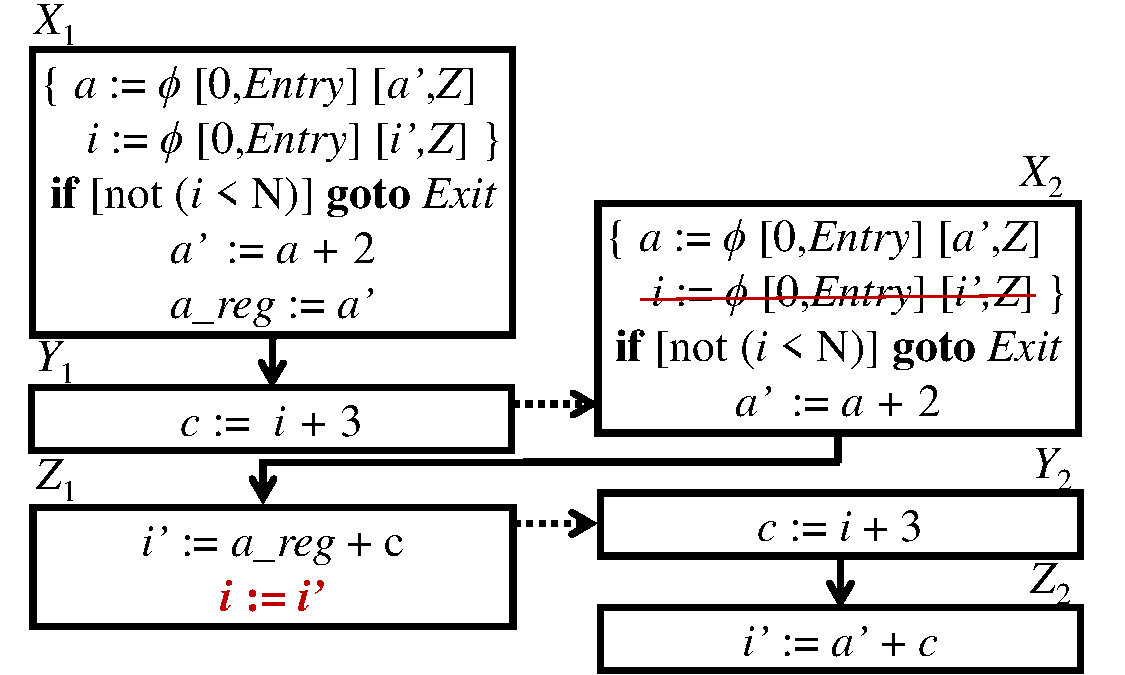
\includegraphics[height=1.7in]{fig-rpe/data-forwarding}
\\
(a) & (b)
\end{tabular}
\end{center}
\caption{(a) Generate Edges for pipelined CCDFG (b) Data propagation.}
\label{fig:algorithm-2}
\end{figure}
 
\item {\bf Generate edges:} The algorithm adds the edges for data and control flow as shown in Figure~\ref{fig:algorithm-2}(a). Control edges are edges from one scheduling superstep to the next. Data forwarding edges forward data from one scheduling step to the next in a single scheduling superstep. Loop edge denotes the repetition of the full pipeline stage. Exit edges are from the scheduling steps to the $Exit$ block. Note, a pipelinable loop has only one $Exit$ block.

\item {\bf Generate data propagation:} In Figure~\ref{fig:algorithm-2}(b), we require the value of $i'$ in $X_2$ to execute the following statement:
$$ i := \phi [0, Entry][i', Z]$$
But, if we execute $X_2$ before executing $Z_1$, the value of $i'$ has not yet been produced. To avoid such a situation, we relocate the assignment statement $i := i'$ to $Z_1$. Note, the assignment statement $i := i'$ is obtained from the $\phi$-statement $i := \phi [0, Entry][i', Z]$ since in sequential execution, we would have entered $X_2$ from $Z$ block.
\end{enumerate}

\section{Challenges}
\label{sec:not-verifiable}

Verifying the correspondence between a sequential design and
its pipelined RTL by traditional verification methods is
challenging.  Loop pipelining is a complex transformation
which introduces temporal overlap of iterations. As a
result, the industrial synthesis tools employ the following
features:

\begin{enumerate}
\item Aggressive scheduling strategies are used to produce a
  new schedule.
\item Order of executions of basic block is different from
that of the sequential design, thus changing control flow.
\item New variables are introduced to get rid of data hazards.
\end{enumerate}

Consequently, mappings between the internal operations of
sequential design and pipelined RTL are destroyed. This renders SEC ineffective because in the absence of mappings, SEC gets reduced to checking
input and output correspondence of designs.
This leads to
state space explosion in large designs. Furthermore, since
the synthesis tool vendor typically does not disclose
the implementation of the transformation, direct
certification of the transformation by theorem proving is
also not possible.

However, one key observation is that it is {\em not necessary} to verify the exact transformation implemented
by the behavioral synthesis tool in order to certify the
correctness of the synthesized pipelined RTL. In
particular, one can create one's own pipelining algorithm, that takes a sequential CCDFG and creates the
pipelined counterpart; we can use the latter as a {\em reference
  model} to perform SEC against the synthesized RTL.
Furthermore, the pipelining algorithm can use the
reports from the behavioral synthesis tool (\eg, values of
pipeline parameters, number of iterations pipelined, etc.)
as guidance in generating the pipeline. If such a
pipelining algorithm can be developed and certified
by theorem proving, then we will have exactly the same
confidence in synthesized RTL as if we had certified the
pipelining algorithm used by behavioral
synthesis.\footnote{Of course the algorithm generating the
  reference model would be simpler, and may fail to generate a pipeline when the synthesis tool can synthesize one using more advanced heuristics.  However, {\em if we can generate a pipelined CCDFG which can be used for SEC with the synthesized RTL}, then that is sufficient for
  certification.}

Hao {\em et al.}'s algorithm
(cf. Section~\ref{subsec:kecheng's algorithm}) is a step in
that direction. In particular, they make use of certain
parameter values gleaned from the reports generated by
behavioral synthesis tool to develop a pipelined reference
model which they could use for SEC against the synthesized
RTL. Nevertheless, their algorithm falls short of the
requirement for a {\em certifiable} algorithm.  In
particular, since their algorithm is not designed with
reasoning in mind, it is non-trivial to certify it as it is.

To understand the complexities involved in mechanical
certification of an algorithm that was not designed
originally with certification in mind, we need to re-visit
the general approach to applying formal reasoning on
software programs.  The typical approach is to break the
program into a number of pieces, prove key lemmas
characterizing the role of each piece, and then chain these
lemmas together into a proof of the correctness of the
entire program. Crucial to this approach, however, is the
requirement that each program piece can be characterized by
a succinct invariant that can be easily verified.  However,
in a program not developed with reasoning in mind,
optimizations typically destroy the structural disciplines
and modularity of the individual program pieces. This makes it
difficult to identify and isolate the components that
actually maintain succinct, interesting invariants.  The
result is that in order to certify such an implementation,
one has to either (1)~restructure the implementation into
one that is more disciplined, and prove the equivalence
between the two, or (2)~come up with very complex
invariants that essentially comprehend how invariants from
each individual piece are conflated together in the
implementation.  Both approaches require extensive human
interaction, resulting in the proverbial euphemism of proofs
of programs being orders of magnitude more complex than the
programs themselves~\cite{liu}.

%% It is common knowledge that certifying a complex algorithm
%% which is not written with reasonis
%% difficult to certify. To certify an algorithm, we divide an
%% algorithm into components such that we can identify
%% predicates which are maintained by various components of the
%% algorithm (property of variables of the algorithm). The
%% complexity of verifying an algorithm comes from the
%% complexity of defining and proving these predicates.  We can
%% choose a simple invariant --- state after completely
%% executing the CCDFG is same before and after the various
%% components of the algorithm. But, since the algorithm has
%% not been written keeping this invariant in mind, the various
%% components of the proposed algorithm do not follow this
%% invariant even though the complete algorithm has this
%% property. The components conflate and it is difficult to
%% entangle them in this case.

%% We can come up with a complex invariant to certify the algorithm. There are approaches to do it such as on-track property. But, it is highly complex. (\hl{A small program has costed people PhD (cite examples)}).

In our work, however, we can ``get away'' without verifying
the specific implementation while still being able to
certify the design generated by behavioral synthesis without
loss of fidelity. The key observation, as above, is that it
is sufficient to develop {\em any} certifiable algorithm
that generates a pipelined CCDFG from a sequential
implementation which can be effectively applied with SEC.
In particular, any certifiable algorithm that has the same
input-output characteristic as Hao {\em et al}.'s algorithm
is sufficient.  Thus, this research focuses on identifying
certifiable primitives and invariants of a loop pipelining
transformation and developing a pipeline generation
algorithm using those primitives, achieving the dual goal of
mechanical reasoning of the algorithm and amenability of the
resulting reference model to SEC.


%% Typical theorem proving does not have flexibility of
%% defining an algorithm. However, in our case, we do not
%% need to certify the same algorithm. We just need a
%% certified algorithm which creates a pipeline reference
%% model structurally similar to pipelined RTL. So, we can
%% design our own certifiable pipeline algorithm which has a
%% natural inclination to be certified by theorem proving.

%Certifying an arbitrary algorithm by theorem proving is not always easy.

%To certify an algorithm by theorem proving,an obvious approach is to identify pre-conditions, post-conditions and the invariants i.e, properties that must remain true for the design before and after the algorithm. 

%In our case, the invariant is obvious from our definition of correctness of the pipelined design (refer section ~\ref{subsec:correctness-defn}). We want that if we begin with the same state, the value of all variables in the state (except local variables in the loop introduced as part of pipeline registers) remains same after completely executing the two designs at run time i.e, for all possible combinations of inputs and paths, the two designs (sequential and pipelined implementations) give the same state after execution.

%The algorithm described above is not designed keeping certification in mind. It does not follow the invariant at any step. Infact, even till the third step of the algorithm, the proposed pipelined design still has some data conflicts which are taken care of by data propogation. So, we do not get an advantage of building our proof on steps in this algorithm. Only after completing all the steps we can claim correct execution.

%So, we attempted to prove this invariant on the whole algorithm, which was the only choice left. Indeed, our original proof attempt was different: we tracked for each variable $v$ the microsteps where it is accessed, and proved that $v$ is read and written in succession on ``corresponding'' microsteps in the sequential and pipelined CCDFGs.  However, this lemma cannot be directly used in the final theorem: different variables are accessed at different microsteps; hence, it is difficult to prove a general property about {\em all} variables by induction on the execution steps.

%A second approach to prove the entire algorithm is to come up with an "ontrack property". We assume that when the algorithm terminates, the invariants hold, otherwise we are on-track to prove the invariants. However, defining and proving an on-track property is not an easy task. (cite examples - anthony fox, hanbing liu, magnus myreen).

%So, certifying an adhoc algorithm is theorem proving can be complex. Typical theorem proving does not have flexibility of defining an algorithm. However, in our case, we have a non-standard application of theorem proving. We do not need to certify the same algorithm. We just need a certified algorithm which follows the criterias described before. So, we can design a pipelining algorithm which has a natural inclination to be certified by theorem proving. 

%We realized that at the crux of a pipeline algorithms in behavioral synthesis, there are three primitives that have the capability of affecting the execution of a pipeline. If we can certify these three primitives to be correct by theorem proving, we can introduce some small tweaks to restructure the proposed algorithm so that each step of the algorithm is a combination of these three primitives. Also, it would allow us to extend this framework to create other certified pipelining algorithms if needed.    

\section{Framework to Develop Certifiable Pipeline Algorithms}
\label{sec:fundamental-tasks}

We have developed a framework of three pipelining primitives to create certifiable pipeline algorithms. The key to our approach is the observation that these primitives are 
%that have the potential to change the execution flow. There may be other optimizations, but these primitives 
both necessary and sufficient to create a simple pipeline from an unrolled loop in behavioral synthesis. If we can certify these primitives individually, we can build on them to create a certifiable pipelining algorithm.

\begin{figure}[t!]
\begin{center}
\begin{tabular}{cccc}
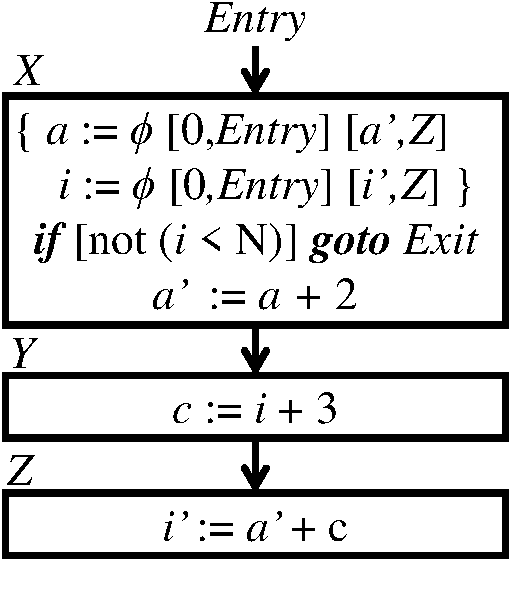
\includegraphics[height=1.4in]{fig-rpe/one-iteration-of-loop}
&
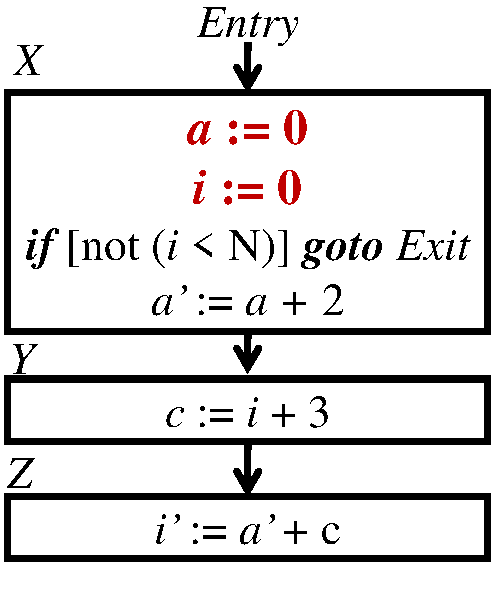
\includegraphics[height=1.4in]{fig-rpe/phi-removal-transformation}
&
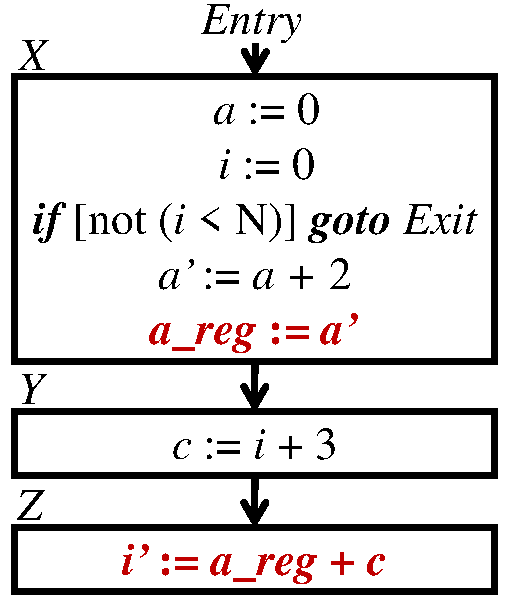
\includegraphics[height=1.4in]{fig-rpe/shadow-register-transformation}
&
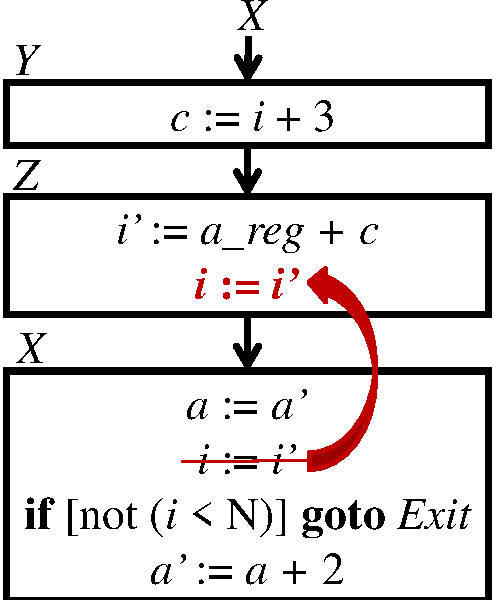
\includegraphics[height=1.4in]{fig-rpe/interchange-transformation}
\\
(a) & (b) & (c) & (d)
\end{tabular}
\end{center}
\caption{(a) First iteration of a loop (b) After $\phi$-elimination primitive (c) After shadow register primitive (d) After interchange primitive}
\label{fig:fundamental-steps}
\end{figure}

\begin{enumerate}
\item \textbf{\emph{$\phi$-Elimination Primitive}}: As mentioned earlier, a $\phi$-construct is a list of $\phi$-statements.
A $\phi$-statement is $v := \phi [\sigma, X] [\tau, Y] $, it executes as $ v := \sigma$ if the statement is reached from $X$ and as $ v := \tau$ if the statement is reached from $Y$. In figure~\ref{fig:fundamental-steps}(b), $i$ gets assigned the value $0$ as the scheduling step before the $\phi$-statement in the first iteration is $Entry$. A $\phi$-statement is used extensively in loops to perform different actions depending on whether the loop body is executed the first time. 

Reasoning about $\phi$-statement is complex since the state depends not only on $s$ but also on the previous scheduling step in the execution history after its execution from state $s$. However, 
we only deal with loops which do not have branching between the scheduling steps. Hence, if we unroll the loop, we can clearly identify a $\phi$-statement and its previous scheduling step in the execution history. So, we can convert each $\phi$-statement to its corresponding assignment statement based on the previous scheduling step in the unrolled loop structure. This primitive is called $\phi$-elimination primitive {\em i.e.,} given the previous scheduling step in the execution history, replace a $\phi$-construct with a list of corresponding assignment statements. 
\begin{gather*}
\{   a := \phi [0, Entry] [a', Z] \\ 
     \,\,\,\,\,\,i := \phi [0, Entry] [i', Z]   \} 
\end{gather*}
The $\phi$-construct given above is replaced with assignment statements given below in Figure~\ref{fig:fundamental-steps}(b).
\begin{gather*}
a := 0 \\
i := 0  
\end{gather*}

\medskip
\item \textbf{\emph{Shadow Register Primitive}}: If a variable $x$ is written in some microstep, then the shadow register primitive allows us to insert a shadow register step after this microstep. A shadow register step is basically the following assignment instruction: 
$$x\_reg := x$$ 
In the shadow register step here, $x\_reg$ is a new shadow variable introduced by the primitive (not part of the state in the original sequential loop). Now, since both $x$ and $x\_reg$ have the same value, the primitive replaces all subsequent reads of $x$ with $x\_reg$ till the next write of $x$. Suppose, the state before executing this step is $s_1$ and after executing is $s_2$, then we have the following relation:

$$ s_2 := s_1 \cup \{ \langle x\_reg, V \rangle \mid V  \text{ is the value of } \allowbreak  x \text{ in } s_1\} $$

As a result, the state with respect to real variables (all variables except shadow registers) is still $s_1$. 
In Figure~\ref{fig:fundamental-steps}(c), we have applied the shadow register primitive to the following microstep: 
$$a' := a + 2$$
We add a shadow register step: 
$$a\_reg := a'$$ 
We then replace the read of $a'$ in $Z$ with $a\_reg$. Note, since we know how each statement executes, we can identify the variables read and written in a statement statically.

\medskip
\item \textbf{\emph{Interchange Primitive}}: If two adjacent microsteps $m$ and $n$ are such that if a variable is written in $m$, it is not read or written in $n$ and vice versa, then we can move $n$ before $m$ without affecting the execution. Also, we can change the scheduling step of a microstep if the order of execution of the microsteps in the CCDFG remains same. In Figure~\ref{fig:fundamental-steps}(d),  
$i := i'$ is first interchanged with $a := a'$ since there is no read-write conflict between the two microsteps. Then, we rearrange the microstep $i := i'$ by moving it from $X$ to $Z$ without affecting the sequence of microsteps. Interchange does not work on microsteps which have a conditional branch statement. We will extend interchange primitive to include these statements in future.

\end{enumerate}
%\item \emph{Superstep construction} -- This operation entails combining the scheduling steps of the successive iterations, forming scheduling ``supersteps'' that act as scheduling steps for the pipelined implementation.  The result for our example is shown in
%Figure~\ref{fig:correctness}(c).  Supersteps must
%account for read-after-write hazards, i.e, if a variable is written in a scheduling step $X$ and read subsequently in
%$Z$ then $Z$ cannot be in a superstep that precedes $X$ in the control/data flow.  Note that we implement data forwarding (forward value of data within a single clock cycle); thus $X$ and $Z$ can be in a single superstep.


	
%\medskip
%\subsection{An ongoing proof of the correctness criterion}
%\label{sec:proof}	
%Our correctness statement naturally breaks into correctness of $\phi$-elimination, shadow register insertion, and superstep construction.
%The $\phi$-elimination theorem reduces to showing that our
%algorithm correctly replaces $\phi$-statements with
%assignments.  Note that this is not trivial since the algorithm has to use static analysis to
%deduce the previous basic block.  Correctness of shadow
%registers requires verifying similar static
%analysis (\eg, to determine the subsequent read of a
%variable after each write. For superstep construction, we need to verify that we can interchange any two adjacent steps which do not have any data dependencies or read-write conflict by static analysis. A series of interchanges can result in a whole block being moved up to create pipeline. 



\section{A Loop Pipeline Algorithm}
\label{sec:pipeline-algo}

We can create a simple certifiable loop pipeline algorithm using the three pipelining primitives. Given a sequential loop $L$ in CCDFG $C$ and pipeline interval $I$, we can create a pipelined loop $L'$ using Algorithm~\ref{algo:disha}. 

Out of these steps, unrolling a loop is a generic compiler transformation. Adding a loop edge is the process of converting an unrolled pipelined loop to a loop which has the back edge in the pipeline full stage to mimic the repetition of the pipeline full stage. Both these steps do not deal with pipelining a loop but merely convert from a loop into its unrolled version and vice versa. We would formalize the proofs of these two steps later. 

\begin{algorithm}[H]
\caption{Certifiable loop pipeline} \label{algo:disha}
\begin{algorithmic}[1]
\Procedure{PipelineLoop}{L, I}
\State $L_1 \leftarrow UnrollLoop (L, I)$.
\State $L_2 \leftarrow \phi-Elimination (L_1) $.
\State $L_3 \leftarrow DataPropagation (L_2) $.
\State $L_4 \leftarrow GenerateShadowRegisters (L_3) $.
\State $ L_5 \leftarrow SuperstepConstruction (L_4) $.
\State $ L' \leftarrow AddLoopEdge (L_5) $.
\State \textbf{return} $(L')$.
\EndProcedure
\end{algorithmic}
\end{algorithm} 

We describe below the steps to convert from an unrolled loop to an unrolled pipelined loop in detail:

\begin{enumerate}
%\item ~Unroll Loop: Unroll loop $L$ by $N / I$ iterations where $N$ is the number of scheduling steps in loop $L$. If the number of scheduling steps is three and pipeline interval is one, we unroll the loop three times. If we pipeline a loop with more that $N / I$ iterations, the pipeline full stage would start repeating.

\item {\bf $\phi$-elimination}: We apply the $\phi$-elimination primitive on an unrolled loop to return a loop in which all the $\phi$-statements have been replaced with their corresponding assignment statements. Figure~\ref{fig:algo1}(a) shows two iterations of the loop for illustration and Figure~\ref{fig:algo1}(b) shows the two iterations after applying the $\phi$-elimination primitive.

\begin{figure}
\begin{center}
\begin{tabular}{ccc}
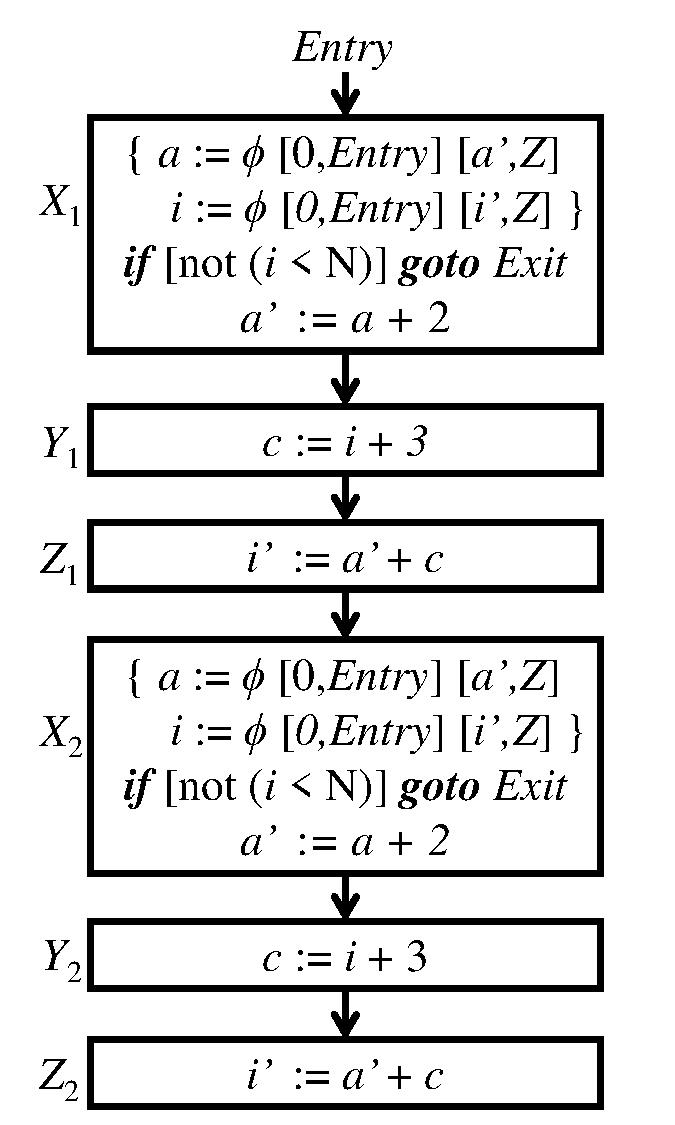
\includegraphics[height=2.5in]{fig-rpe/algorithm-two-iterations}
& 
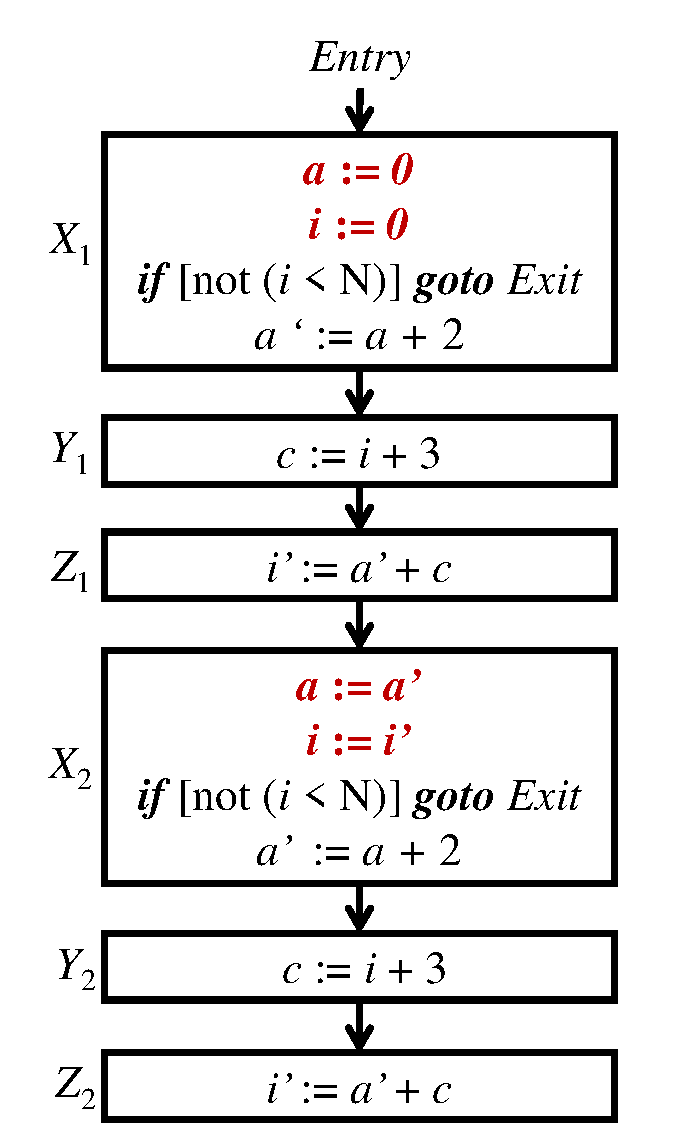
\includegraphics[height=2.5in]{fig-rpe/algorithm-after-phi-elimination}
& 
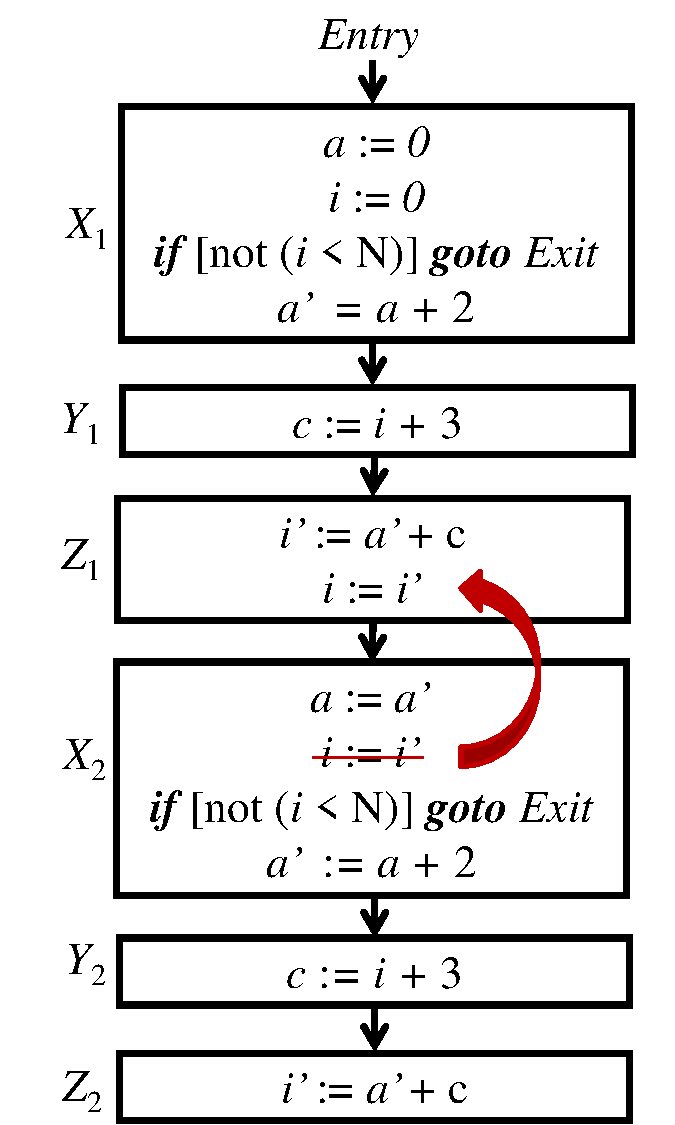
\includegraphics[height=2.5in]{fig-rpe/algorithm-after-data-propagation}
\\
(a) & (b) & (c)
\end{tabular}
\end{center}
\caption{(a) Two iterations of a loop (b) After $\phi$-elimination transformation (c) After data propagation}
\label{fig:algo1}
\end{figure}

\item {\bf Data propagation:} Algorithm~\ref{algo:data-propagation} describes how to compute candidates for data propagation across pipeline iterations. It is a critical step in 


\begin{algorithm}
\caption{Data propagation} \label{algo:data-propagation}
\begin{algorithmic}[1]
\Procedure{DataPropogration}{$L$}
\State $msteps \leftarrow GetLoopCarriedDependencies(L)$.
\For {\textbf{each} mstep \textbf{in} msteps}
 \If {$CheckConflict (L, mstep, N, I) \neq 0$}
\State $L \leftarrow RelocateMStep (L, mstep)$.
\EndIf
\EndFor
\State \textbf{return} $(L)$.
\EndProcedure
\end{algorithmic}
\end{algorithm}

removing data hazards. We want to make sure that when we pipeline a loop, we do not read a variable which has not yet been written. A critical observation is that data propagation is required only for loop carried dependencies.
$GetLoopCarriedDependencies$ identifies the microsteps where loop carried dependencies are being read. Then, $CheckConflict$ checks whether there would be a conflict when we would pipeline the loop. 
%This can be achieved by checking whether the value read in a microstep is written anywhere in the previous $N - I$ \hl{explain} scheduling steps. 
If so, $RelocateMSteps$ relocate the microstep which reads the variable in an iteration to immediately after the microstep which last writes the variable in the previous iteration to remove the conflict. In Figure~\ref{fig:algo1}(c) we found that the loop carried dependency $i'$ in $X_2$ would create a conflict when we would move $X_2$ before $Z_1$ while pipelining. So, we relocate the microstep $i := i'$ after the microstep $i' := a' + c$. Note, $RelocateMStep$ can be seen as an application of a series of interchange primitives. We can only move a microstep upwards till there is no read-write conflict. 

\begin{figure}[t!]
\begin{center}
\begin{tabular}{cc}
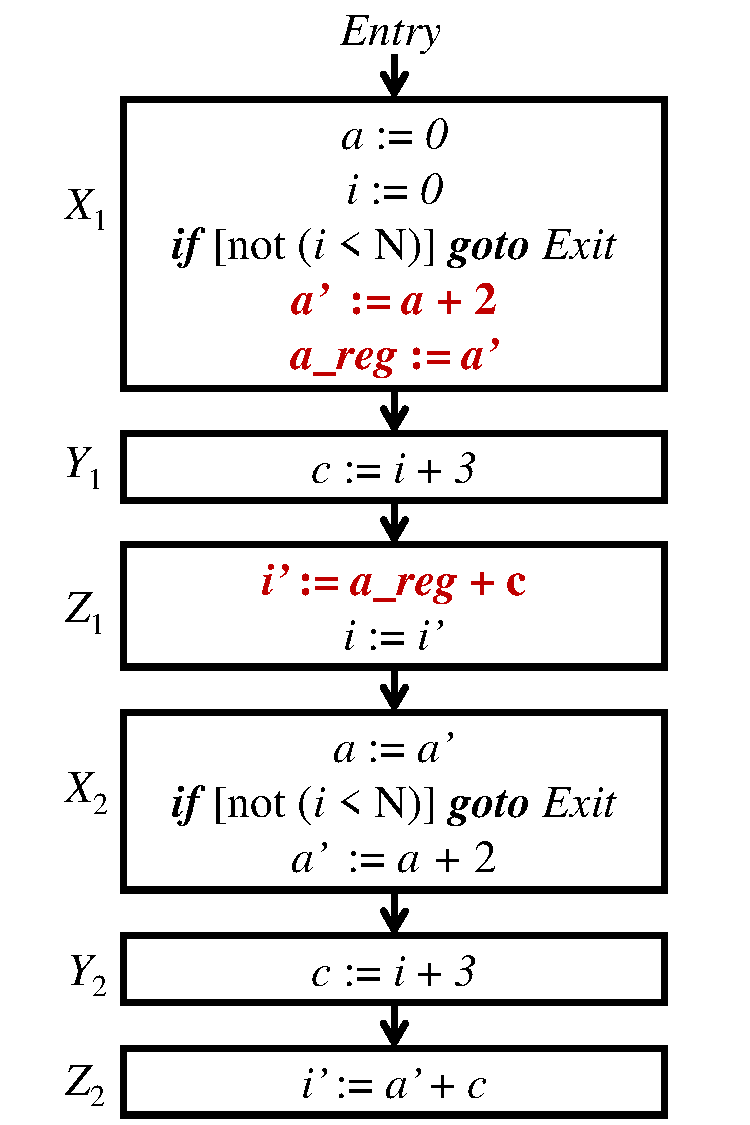
\includegraphics[height=2.5in]{fig-rpe/algorithm-after-shadow-register}
&
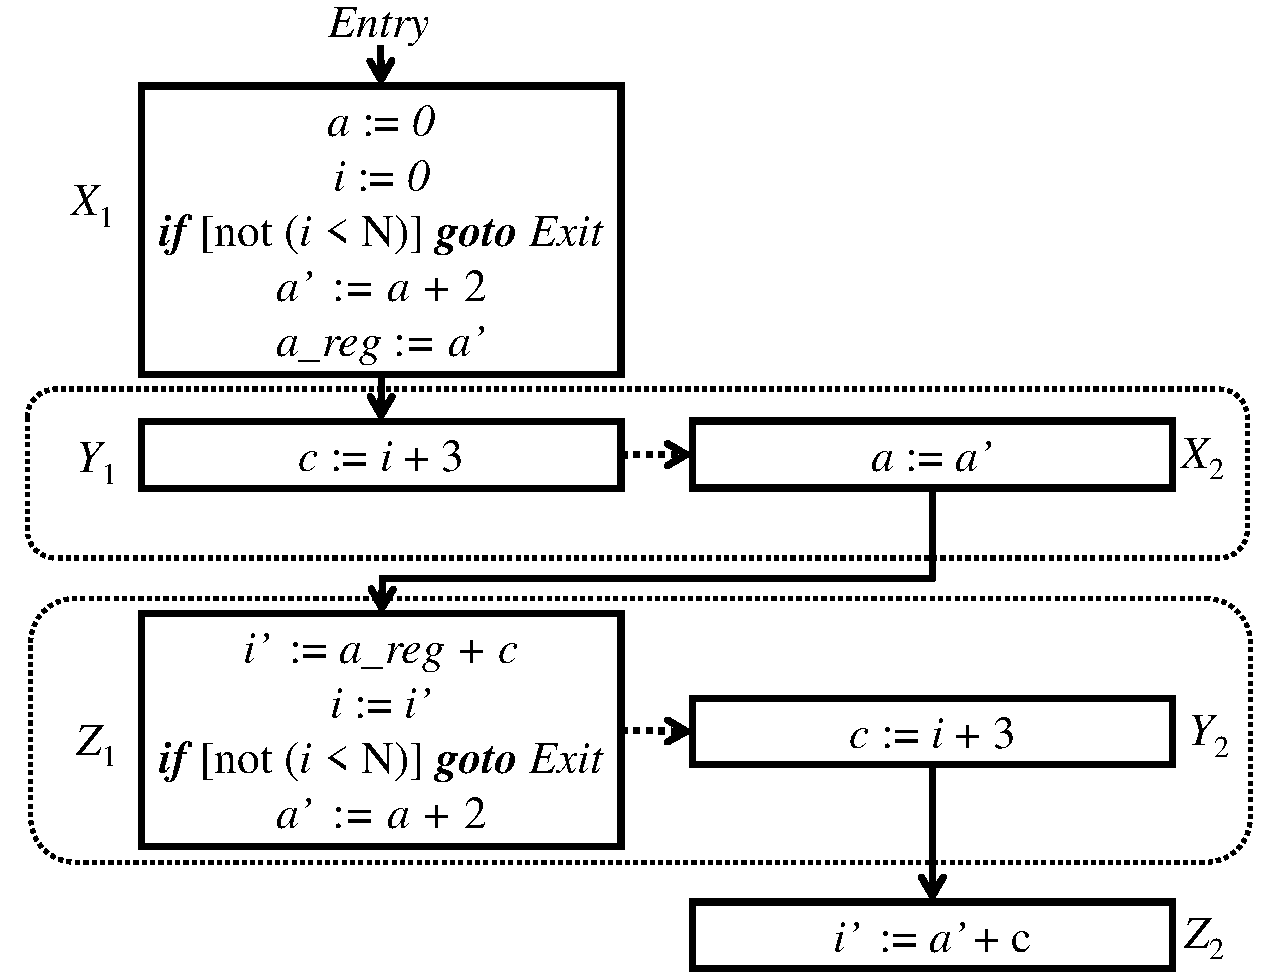
\includegraphics[height=2.5in]{fig-rpe/algorithm-after-superset-construction}
\\
(a) & (b)
\end{tabular}
\end{center}
\caption{(a) After shadow register (b) After superstep construction}
\label{fig:algo2}
\end{figure}

\begin{algorithm}
\caption{Generate shadow registers} \label{algo:generate-pipeline-registers}
\begin{algorithmic}[1]
\Procedure{GenerateShadowRegisters}{$L$}
\State $V \leftarrow GetAllVariables(L)$.
\For {\textbf{each} v \textbf{in} V}
\State $w_v \leftarrow WriteVariable (v, L)$.
\State $r_v \leftarrow LastReadVariable (v, L)$.
%\State $y \leftarrow RequireShadowRegister (r_v, w_v, I)$.
  \If {$RequireShadowRegister (r_v, w_v, I) \neq 0$} 
\State $L \leftarrow AddShadowRegister (w_v, L)$.
\EndIf
\EndFor
\State \textbf{return} $(L)$.
\EndProcedure
\end{algorithmic}
\end{algorithm}

\item {\bf Generate shadow registers:} Algorithm~\ref{algo:generate-pipeline-registers} inserts shadow registers to prevent variables from being overwritten before being read. We first compute all program variables that may be overwritten before being read, which means these are the variables that require shadow registers. To find such variables, $GetAllVariables$ first gets a set of all variables. Then, for each variable, we compare the distance between the write of the variable $w_v$ $(WriteVariable)$ and the last read of the variable $r_v$ $(LastReadVariable)$ in an iteration; if the distance is greater than $I$, %variable is assigned the new data value of the next iteration before current iteration’s value has been fully consumed; this warrants insertion of pipeline variables in every scheduling step between the $r_v$ and $w_v$. The value is propagated every clock cycle following the CCDFG data flow. 
we apply the shadow register primitive on the microstep which writes the variable $(AddShadowRegister)$. We assign that variable to a new variable called shadow register and replace all subsequent reads of that variable with the shadow register till its next write. In Figure~\ref{fig:algo2} (a), we introduce a shadow register $a\_reg$ in iteration 1.
   
\item {\bf Superstep construction:} Now that we have removed the data hazards, we can successfully pipeline the loop using the pipeline interval $I$. We combine the scheduling steps of the successive iterations, forming scheduling ``supersteps'' that act as scheduling steps for the pipelined
implementation. For example, if there are three scheduling steps and the pipeline interval is one, then the unrolled loop structure has nine scheduling steps from ${1 \ldots 9}$. When we pipeline the loop, we have to construct new scheduling steps ${s_1, s_2, \ldots}$ such that $1$ is in $s_1$, $2$ and $4$ are in $s_2$, $3$, $5$ and $7$ are in $s_3$ and so on resembling the pipelined loop structure.
Supersteps must account for read-after-write hazards, i.e, if a variable is written in a scheduling step $s$ and read subsequently in
$s'$ then $s'$ cannot be in a superstep that precedes $s$ in the control/data flow. A scheduling step is allowed to move up another scheduling step only if there are no intermediate read and write conflicts. Note that we implement data forwarding; thus $s$ and $s'$ can be in a single scheduling superstep. 
%Therefore, this step is a  function takes two basic blocks numbers as input, makes sure that there are no read-after-write hazards if we move the second block just before and The result for our example is shown in
%Fig.~\ref{fig:algo2}(b).  
%ConstructSuperstep (x, y) is created by a series of MoveUp operations for each mstep in the scheduling step $x$ such that they reach the position below $y$ if there are no read-write conflicts. 
In Figure~\ref{fig:algo2}(b), scheduling steps $X_2$ and $Z_1$ have no read write conflict now, so we can move step by step the microsteps of $X_2$ using the interchange primitive before $Z_1$. Note, since currently we do not interchange the microstep which has the conditional branch, all the microsteps including and after the conditional branch in $X_2$ do not move above $Z_1$. As part of future work, we would include the conditional branch in the interchange primitive.

%\begin{algorithm}
%\caption{Superstep Construction} \label{algo:superstep-construction}
%\begin{algorithmic}[1]
%\Procedure{SuperstepConstruction}{$L_3$, $N$, $I$}
%\For b 1 to (N - 1)
%\For a 1 to N
%\State $L_3 \leftarrow ConstructSuperstep (a + (N * b), a + (N / I * b))$.
%\State $L_3 \leftarrow ConstructSupersteps (L_3, N, I)$
%\State $L_4 \leftarrow RenameSchedulingSteps (L_4)$.
%\EndFor
%\EndFor
%\State \textbf{return} $(L_4)$.
%\EndProcedure
%\end{algorithmic}
%\end{algorithm}

%\item ~AddLoopEdge --- We add the loop edge (work with Sandip on justification of this step).

\end{enumerate}

It can be seen that the each step in the process to convert an unrolled loop into its pipelined counterpart is a combination of our three primitives. Next, we discuss an outline of the proof of the three primitives using theorem proving.

%\medskip
%\begin{algorithm}
%\caption{Unroll Loop} \label{algo:unroll-loop}
%\begin{algorithmic}[1]
%\Procedure{UnrollLoop}{L, I}
%\State $L_1 \leftarrow \emptyset$.
%\State $N \leftarrow FindNumberOfBlocks (L)$.
%\State $i \leftarrow 0$.
%\While {$i \leq N/I $}
%\State $L_1 \leftarrow AddLoopIteration (L_1)$.
%\State $i \leftarrow i + 1$. 
%\EndWhile 
%\State \textbf{return} $(L_1)$
%\EndProcedure
%\end{algorithmic}
%\end{algorithm}

 
\section{Mechanized Proof Using Theorem Prover}
\label{sec:proof}

Correctness of loop pipelining algorithm using our framework naturally breaks
down into correctness of $\phi$-elimination, shadow register and interchange primitives. For each of these three primitives, mechanical certification has two aspects:

\begin{enumerate}
\item {\bf Correctness of primitive:} We must prove that
  applying a particular primitive is correct, {\em i.e.},
  maintains a certain invariant.  This is proven without
  considering how it is applied in the context of a pipeline
  synthesis algorithm.  For example, for the interchange
  primitive, we prove that starting with the same state $s$,
  executing two microsteps in sequence produces the same
  state as executing the same microsteps in interchanged
  order.  Note that this is independent of how the primitive
  is actually applied during pipelining.
 
\item {\bf Correctness of primitive application :} This
  step is to show that the primitive is applied by our
  algorithm properly, {\em i.e.}, the environment
  assumptions where the {\bf Correctness of primitive}
  depends are maintained appropriately by the algorithm at
  the point where the primitive is applied.  

%% How to set up the Inductive proof
%%   to ensure correctness of CCDFG after applying a primitive:
%%   We prove that execution of the entire CCDFG is not changed
%%   when the primitive is applied. Also, we need to statically
%%   ensure that the function we have created to apply the
%%   primitive is correct.
\end{enumerate}

\medskip
\noindent {\bf Correctness of primitive:} We give an outline of the proof to justify that the three primitives are correct.

\begin{enumerate}
\item {\bf $\phi$-elimination primitive:} We prove that execution
  of a $\phi$-construct is same as executing corresponding
  assignment statements. Note that this is not trivial since
  given a microstep in a scheduling step containing the
  $\phi$-construct, the algorithm has to use static analysis
  to deduce the previous scheduling step.

\item {\bf Shadow register primitive:} We prove that adding
  a shadow register microstep $x\_reg = x$ does not change the
  value of any variable except the shadow variable. Also, we
  prove that now since value of $x\_reg$ would be equal to value
  of $x$, executing a statement which reads $x$ has same
  effect on the state as executing a statement which reads
  $x\_reg$ till the next write of $x$. As mentioned earlier, we
  determine the variables read and written in a statement by
  analyzing the execution semantics.

\item {\bf Interchange primitive:} We want to prove that we can interchange two microsteps which do not have
  read-write conflict. Given an initial state, the state after
  executing microsteps $m$ and $n$ is the same as the state after
  executing $n$ then $m$ if $m$ and $n$ have no read-write
  conflict. Suppose, state after
  executing $m$ and $n$ is $s_1$ and after executing $n$ and
  $m$ is $s_2$. We prove that for any variable $x$, its
  value remains same in $s_1$ and $s_2$.  After normalizing
  the states, we can prove that $s_1$ is equal to $s_2$ i.e,
  states remain same after executing the two microsteps in
  sequence or in an interchanged order. Again, reasoning about read and
  write of statements involves reasoning about execution
  semantics of all types of microsteps present in the
  language which is not trivial.
\end {enumerate}

\medskip
\noindent {\bf Correctness of primitive application:} The
correctness of each primitive discussed above, entails a
so-called ``assume-guarantee'' reasoning: the prmitive is
guaranteed to maintain the desired invariant if and only if
it is applied under certain well-formed conditions.  To use
these correctness statements to verify the algorithm, we
must therefore prove that the algorithm applies each
primitive appropriately, maintaining the well-formedness
condition required for the correctness of the primitive.

Note that verifying this requires an inductive proof
relating the states of the CCDFG $C'$ generated after the
application of the transformation with the original CCDFG
$C$.  The induction is on the lengths of execution of $C$
and $C'$.  Note that the induction is non-trivial because
transformations have significant ``global'' effect on a
CCDFG.  These include one or more of the following:

\begin{enumerate}
\item replacing one microstep of $C$ with more than one
  microsteps in $C'$ ({\em e.g.}, $\phi$-elimination), or
\item interchanging several microsteps ({\em e.g.},
  interchange), or
\item changing the variable being read or written in several
  microsteps ({\em e.g.}, shadow register)
\end{enumerate}
The upshot is that an inductive theorem relating $C$ and
$C'$ must be strong enough to comprehend the global effects.
For instance, an inductive statement showing the
correctness of $\phi$-elimination must account for the fact
that the number of microsteps of $C$ is different from that
of $C'$.  Thus an execution of $C$ for $n$ microsteps must
correspond to an execution of $C'$ for a different number
$m$ of microsteps, where the number $m$ is a function of $n$
and the structures of $C$ and $C'$; the statement of the
correctness of $\phi$-elimination must characterize the
value of $m$ precisely, perhaps defining functions that
statically and symbolically execute $C$ and $C'$, in order
to be provable by induction.  Furthermore the functions so
introduced for static symbolic execution must themselves be
proven correct.

%% \begin{enumerate}
%% \item Phi Elimination: Note that a $\phi$-construct
%%   decomposes into one or more assignment statements. So, the
%%   number of total microsteps in $C_2$ is more than or equal
%%   to microsteps in $C_1$.  

%% Inductive hypothesis: Executing n microsteps of $C_1$ is equal to executing some corresponding f(n) microsteps of $C_2$. f(n) can be derived from n by statically analyzing number of $\phi$-statements in $C_1$.

%% Induction base case: Executing $0$ microsteps of $C_1$ is equal to executing $f(0) = 0$ microsteps of $C_2$. This is trivially true as both start from the same state $s$.
 
%% Inductive step: Prove that executing $n + 1$ microsteps of $C_1$ is equal to executing $f(n + 1)$ microsteps of $C_2$. We can prove that executing $n + 1$ microsteps is equal to executing $n$ microsteps and then executing $(n + 1)th$ step. So, this proof can be split into two cases.
  
%% \begin{itemize}
%% \item Case I: The microstep at $(n + 1)$ level is not a $\phi$-construct. Then, we need to prove that microstep at $(n + 1)$ level in $C_1$ is same as microstep at $f(n + 1)$ level in $C_2$ and their execution produces same result.
%% %$$ f(n + 1) = f(n) + 1 $$.

%% \item Case II: The microstep at $(n + 1)$ level is a $\phi$-construct. Then, we need to prove that there are corresponding assignment statements between $f(n)$ and $f(n + 1)$ level. Then, we use the proof of the phi elimination primitive discussed earlier that execution of $\phi$-construct is same as execution of corresponding assignment statements.
%% \end{itemize}

%% \item Shadow Register --- Let $m$ be the microstep in $C_1$ which writes the variable $v$ which may be overwritten while pipelining. So, the primitive adds a shadow register step after $m$ in $C_2$, say $$ vr = v$$ where $vr$ is a shadow variable. Let the last step that reads $v$ be $l$. Suppose total number of microsteps in $C_1$ is $k$, then $C_2$ has $k + 1$ microsteps because shadow register primitive adds one step (shadow register step).

%% $$ k = a + (k - a - b)+ b $$
%% where $a$ is the number of microsteps upto and including microstep $m$ and $b$ is the number of microsteps after microstep $l$.

%% \begin{itemize}
%% \item Case I: Executing $n$ microsteps in $C_1$ is equal to executing $n$ microsteps in $C_2$ where $n \leq a$.

%% Base Case: $n = 0$. This is trivially true as both start from the same state $s$.

%% Inductive hypothesis: Executing $n - 1$ microsteps in $C_1$ is equal to executing $n - 1$ microsteps in $C_2$ where $n <= a$.

%% Induction Step: Prove that executing $n$ microsteps of $C_1$ is equal to executing $n$ microsteps of $C_2$. We can prove that executing $n $ microsteps is equal to executing $n - 1$ microsteps and then executing step at $n$ level. So, for this proof, we need to prove that the step at level $n$ for any $n \leq a$ is same in both $C_1$ and $C_2$.

%% \item Case II: Executing $n$ microsteps in $C_1$ is equal to executing $n + 1$ microsteps in $C_2$ where $ a < n <= b $.

%% We know, step at level $(a + 1)$ in $C_2$ is a shadow register step which does not change the state with respect to real variables. After that, we have two cases:

%% Case I: The step at level $n$ of $C_1$ is equal to the step at level $(n + 1)$ of $C_2$.

%% Case II: Shadow register primitive replaces read of variable $v$ in the step at level $n$ of $C_1$ with $vr$ in the $(n + 1)$ step of $C_2$ which does not affect execution.

%% \item Case III: Executing $n$ microsteps in $C_1$ is equal to executing $n + 1$ microsteps in $C_2$ where $n \geq b$.

%% Base Case: $n = b$. This is proved by Case II.

%% Inductive hypothesis: Executing $n - 1$ microsteps in $C_1$ is equal to executing $n$ microsteps in $C_2$ where $n > b$.

%% Induction Step: Prove that executing $n$ microsteps of $C_1$ is equal to executing $n + 1$ microsteps of $C_2$. We know that executing $n $ microsteps is equal to executing $n - 1$ microsteps and then executing the step at level $n$. So, we need to prove that
%% the step at level $n$ in $C_1$ is equal to the step at level $(n+1)$ in $C_2$ for n > b. 
%% \end{itemize}

%% \item Interchange: Let $m$ and $n$ be the two microsteps in $C_1$ which are adjacent and have no read-write conflict. Suppose total number of microsteps in $C_1$ is $k$, then $C_2$ also has $k$ microsteps because interchange primitive does not add or remove any microsteps.
%% $$ k = i + 2 + (k - i - 2) $$
%% where $i$ is the number of microsteps before microstep $m$ and $k - i - 2$ is the number of microsteps after microstep $n$.

%% \begin{itemize}
%% \item Case I: Executing $n$ microsteps in $C_1$ is equal to executing $n$ microsteps in $C_2$ where $n \leq i$.

%% Base Case: $n = 0$. This is trivially true as both start from the same state $s$.

%% Inductive hypothesis: Executing $n - 1$ microsteps in $C_1$ is equal to executing $n - 1$ microsteps in $C_2$ where $n \leq i$.

%% Induction Step: Prove that executing $n $ microsteps of $C_1$ is equal to executing $n $ microsteps of $C_2$. We know that executing $n $ microsteps is equal to executing $n - 1$ microsteps and then executing the step at level $n$. So, to prove that states after executing $n$ microsteps are equal, we need to prove that for any $n \leq i$, the step at level $n$ both $C_1$ and $C_2$ are same.

%% \item Case II: Executing $i + 2$ microsteps in $C_1$ is equal to executing $i + 2$ microsteps in $C_2$.

%% We know, $m$ is the microstep at level $(i + 1)$ in $C_1$ and $n$ is the microstep at $(i + 2)$ level. We also know that executing $ i + 2 $ microsteps is equal to first executing $i $ microsteps and then executing $2$ microsteps after that. Since, Case I proves that executing $i$ microsteps is equal in $C_1$ and $C_2$, we are left with one case:
%% To prove that the two microsteps after $i$ level in $C_2$ are $n$ and $m$. This can be proved as we have proved earlier that executing $m$ followed by $n$ is same as executing $n$ followed by $m$ if there are no-read write conflicts between $n$ and $m$
%% (proof of interchange primitive).

%% \item Case III: Executing $n$ microsteps in $C_1$ is equal to executing $n$ microsteps in $C_2$ where $n \geq i + 2$.

%% Base Case: $n = i + 2$. This is proved by Case II.

%% Inductive hypothesis: Executing $n - 1$ microsteps in $C_1$ is equal to executing $n - 1$ microsteps in $C_2$ where $n > i + 2$.

%% Induction Step: Prove that executing $n $ microsteps of $C_1$ is equal to executing $n $ microsteps of $C_2$. We know that executing $n $ micro is equal to executing $n - 1$ microsteps and then executing the step at level $n$. So, to prove that states after executing $n$ microsteps are equal, we need to prove that for any $n > i + 2$, the step at level $n$ in both $C_1$ and $C_2$ is same.

%% <<<<<<< .mine
%% %% \end{itemize}
%% %% \end{enumerate}
%% %% \medskip
%% %% \bf{Proof progress}
%% %% %\label{subsec:proof-progress}
%% =======
%% \end{itemize}
%% \end{enumerate}
%% \medskip
%% \em {\bf {Proof progress}}
%% %\label{subsec:proof-progress}
%% >>>>>>> .r36

At the time of this writing, we have (1)~developed a
framework to create certifiable pipelining algorithms (2)~created a
certifiable algorithm to generate a pipeline reference model
using feedback from the tool and our three design primitives
(3)~completed the proof for correctness of the three
primitives. (4)~substantially completed the inductive proof
of correctness of application for $\phi$-elimination and
interchange primitives using ACL2 theorem prover~\cite{car}.
 
We expect the proofs of other induction operations to be
similar since their definition involves similar static analysis. Our formalization involves
$186$ definitions. About $350$ mechanically checked
lemmas are involved in the proofs that have been completed.

\section{Related Work}
\label{sec:related}

There has been significant research on formal verification of correctness of pipeline. Most of this research has
focused on pipelines in processors~\cite{bd:pipeline,bt:pipeline,sh:pipeline,pm:pipelines,rh:pipelines,aagard-day:compare}.
%~\cite{aagard-day:compare} 
%provide a comprehensive overview of this work.
Our work has similarities in formalization of pipelines. However, there is a difference in requirements due to the domain of application. In particular, while processor pipelines require proof of correspondence
between a single sequential design and its pipelined
counterpart, our work targets an algorithm for synthesizing pipelined designs. On one hand, our verification problem is harder since it
focuses on a synthesis algorithm rather than an individual
design.  On the other hand, since we are using a simple algorithm with no optimizations, our pipelined design is simpler as compared to a synthesized pipelined design.

Our work has parallels in software pipelines as well. Recently, Tristan and Leroy~\cite{tl:software-popl10}
present a verified translation validator for software loop
pipelines: their algorithm checks that a pipelined
loop is equivalent to the sequential counterpart. However,
their correctness statement is contingent upon the equivalence of symbolic simulation of the two designs.
%\hl{Read this paper http://dl.acm.org/
%citation.cfm?id=1542513}.
\section{Conclusion and Future Work}
\label{sec:concl}

To certify behaviorally synthesized pipelined designs, we require a certifiable loop pipelining algorithm to generate a pipeline reference model. The reference model can then be compared with pipelined RTL generated by industrial synthesis tools using SEC. We have identified three pipelining primitives to create certifiable pipelining algorithms. We have also shown how to create a simple certifiable loop pipelining algorithm in behavioral synthesis using our primitives. 

We need to expand the interchange primitive to include the microstep with a conditional branch. The proof of the three primitives is still a work in progress. Also, we need to formalize the proof for converting an unrolled pipelined loop to a pipelined loop with a loop edge. We believe our framework can be extended to algorithms with complicated heuristics as well. In future, we would also explore the possibility of extending this to function pipelines.


\bibliographystyle{splncs}
\bibliography{bib}
\end{document}
